% !TeX root = surprises.tex

\selectlanguage{hebrew}


\chapter[\R{האם משולשים עם אותו שטח ואותו היקף חופפים?}]{האם משולשים עם אותו שטח\\
ואותו היקף חופפים?}
\label{c.congruent}
%%%%%%%%%%%%%%%%%%%%%%%%%%%%%%%%%%%%%%%%%%%%%%%%%%%%%%%%%%%%%%%


האם משולשים עם אותו שטח ואותו היקף חופפים? לא בהכרח: לשני המשולשים הלא-חופפים עם הצלעות
$(17,25,28)$
ו-%
$(20,21,27)$
היקף
$70$
ושטח 
$210$
(איור%
~\ref{f.congruent-first-example}).
פרק זה מראה שנתון משולש עם אורכי צלעות רציונליים, ניתן לבנות משולש לא-חופף עם אורכי צלעות רציונליים, ועם אותו היקף ושטח.
בסוף הפרק הבאתי הוכחה אלגנטית לנוסחה של הרון לשטח של משולש. את השיטה נדגים על דוגמה ונראה שלמשולש עם הצלעות 
$(3,4,5)$
ולמשולש עם הצלעות
$(\frac{156}{35},\frac{101}{21},\frac{41}{15})$
אותו היקף
$12$
ואותו שטח
$6$.

\begin{figure}[htb]
\begin{center}
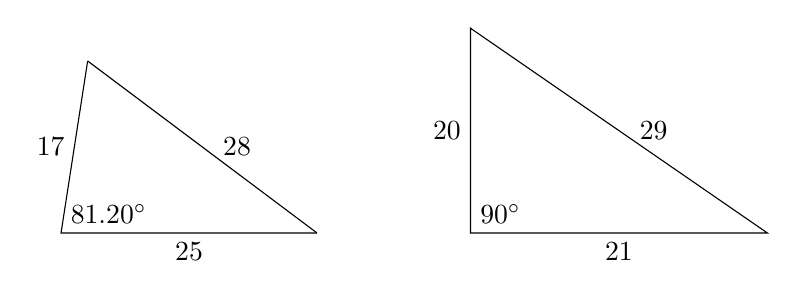
\begin{tikzpicture}[scale=1.3]
\coordinate (A1) at (0,0);
\node[above right] at (A1) {$81.20^\circ$};
\coordinate (B1) at (2.5cm,0);
\coordinate (C1) at (81.20:1.7cm);
\draw (B1) -- node[below] {$25$} (A1) -- node[left] {$17$} (C1);
\draw (B1) -- node[right,xshift=4pt] {$28$} +(143.13:2.8cm);
\begin{scope}[xshift=4cm]
\coordinate (A2) at (0,0);
\node[above right] at (A2) {$90^\circ$};
\coordinate (B2) at (2.9cm,0);
\coordinate (C2) at (0,2cm);
\draw (B2) -- node[below] {$21$} (A2) -- node[left] {$20$} (C2) -- node[right,xshift=4pt] {$29$} cycle;
\end{scope}
\end{tikzpicture}
\end{center}
\caption{משולשים לא חופפים עם אותו שטח ואותו הקיף}\label{f.congruent-first-example}
\end{figure}


\section{ממשולש לעקומה אליפטית}

נתון משולש עם קודקודים
$A,B,C$
וצלעות
$a,b,c$,
חוצי הזוויות נפגשים בקודה אחת
$O$
שהוא המרכז של מעגל החסום על ידי המשולש )איור~%
\ref{f.inscribed}(.%
\footnote{במעגל חסום וצלעות משיקים למעגל והעובדה שהם חוצי הזוויות נובעת מהתכונות של משיקים.}
$OA',OB',OC'$
הם הגבהים של המשולש. באיור סומנו גם זוגות של זוויות מרכזיות
$\alpha/2,\beta/2,\gamma/2$.
השוויון של הזוויות נובע ממשולשים ישר-זווית חופפים:
\[
\triangle AOB'\cong \triangle AOC',\quad \triangle BOA'\cong \triangle BOC', \quad \triangle COA'\cong \triangle COB'\,.
\]
החפיפת המשולשים מתקבל גם שוויון בין קטעי הקו 
$u,v,w$
המחברים את הצלעות עם נקודת ההשקה שלהן עם המעגל.



\begin{figure}[htb]
\begin{center}
\begin{tikzpicture}[baseline=-6mm,scale=2.25]
% Draw base and path two lines at known angles
\draw (0,0) coordinate (a) node[xshift=-6pt] {$A$} -- (0:6) coordinate (b) node[xshift=6pt] {$B$};
\path[name path=ac] (a) -- +(50:4);
\path[name path=bc] (b) -- +(150:5);
% Get their intersection and draw lines between vertices
\path[name intersections={of=ac and bc,by=c}];
\node[above] at (c) {$C$};
\draw (a) -- (c) -- (b) -- (a);
% Label angles with tick marks
\draw (a) ++(0:4mm) arc (0:50:4mm);
\draw (a) ++(10:3.5mm) -- +(10:1mm);
\draw (a) ++(15:3.5mm) -- +(15:1mm);
\draw (a) ++(35:3.5mm) -- +(35:1mm);
\draw (a) ++(40:3.5mm) -- +(45:1mm);
\draw (b) ++(150:5mm) arc (150:180:5mm);
\draw (b) ++(157.5:4.5mm) -- +(157.5:1mm);
\draw (b) ++(172.5:4.5mm) -- +(172.5:1mm);
\draw (c) ++(230:3mm) arc (230:330:3mm);
\draw (c) ++(250:2.5mm) -- +(250:1mm);
\draw (c) ++(255:2.5mm) -- +(255:1mm);
\draw (c) ++(260:2.5mm) -- +(260:1mm);
\draw (c) ++(300:2.5mm) -- +(300:1mm);
\draw (c) ++(305:2.5mm) -- +(305:1mm);
\draw (c) ++(310:2.5mm) -- +(310:1mm);
% Path bisectors of two lines
\path[name path=bia] (a) -- +(25:3.5);
\path[name path=bib] (b) -- +(165:5);
% Intersection of angle bisectors
\path [name intersections={of=bia and bib,by=center}];
% Draw angle bisectors to center
\draw (a) -- (center);
\draw (c) -- (center);
\draw (b) -- (center);
% Draw radii
\draw (center) -- node[left] {$r$} ($(a)!(center)!(b)$) node[below,yshift=-2pt] {$C'$} coordinate (ap);
\draw (center) -- node[left,yshift=-4pt] {$r$} ($(a)!(center)!(c)$) node[above left] {$B'$} coordinate (bp);
\draw (center) -- node[right] {$r$} ($(b)!(center)!(c)$) node[above right] {$A'$} coordinate (cp);
% Draw dots
\fill (center) circle (.5pt) node[above,xshift=3pt,yshift=6pt] {$O$};
\fill (a) circle (.5pt);
\fill (b) circle (.5pt);
\fill (c) circle (.5pt);
\fill (ap) circle (.5pt);
\fill (bp) circle (.5pt);
\fill (cp) circle (.5pt);
% Draw right angle squares
\draw (ap) -- ++(90:4pt) -- ++(0:4pt) -- ++(-90:4pt);
\draw (bp) -- ++(-40:4pt) -- ++(-130:4pt) -- ++(-220:4pt);
\draw (cp) -- ++(-30:4pt) -- ++(-120:4pt) -- ++(-210:4pt);
% Labels of angles
\node[above,xshift=5pt,yshift=21pt] at (center) {$\gamma/2$};
\node[above left,xshift=-4pt,yshift=21pt] at (center) {$\gamma/2$};
\node[above right,xshift=4pt,yshift=-5pt] at (center) {$\beta/2$};
\node[below right,yshift=-6pt] at (center) {$\beta/2$};
\node[left,xshift=-8pt,yshift=3pt] at (center) {$\alpha/2$};
\node[below left,xshift=2pt,yshift=-6pt] at (center) {$\alpha/2$};
% Labels of line segments (names of points are weird...)
\path (a) -- node[below,yshift=-2pt] {$u$} (ap);
\path (a) -- node[left, xshift=-2pt] {$u$} (bp);
\path (b) -- node[above,yshift=2pt]  {$v$} (cp);
\path (b) -- node[below,xshift=-2pt] {$v$} (ap);
\path (c) -- node[above,xshift=-2pt] {$w$} (bp);
\path (c) -- node[above,xshift=2pt]  {$w$} (cp);
% Labels of sides
\draw[<->] ($(a)+(0,-15pt)$) -- node[fill=white] {$c$} 
           ($(b)+(0,-15pt)$);
\draw[<->] ($(a)+(-12pt,10pt)$) -- node[fill=white] {$b$}
           ($(c)+(-12pt,10pt)$);
\draw[<->] ($(b)+(6pt,13pt)$) -- node[fill=white] {$c$}
           ($(c)+(6pt,13pt)$);
% Inscribed circle
\node[thick,dotted,draw,circle through=(ap)] at (center) {};
\end{tikzpicture}
\end{center}
\selectlanguage{hebrew}
\caption{מעגל חסום המוגדר על ידי חיתוך חוצי הזווית משולש}\label{f.inscribed}
\end{figure}



השטח 
$S_{\triangle ABC}$
הוא סכום השטחים של 
$\triangle AOC, \triangle BOC, \triangle AOB$:

\begin{eqnlabels}
S_{\triangle ABC} &=& \frac{1}{2}(w+v)r + \frac{1}{2}(v+u)r + \frac{1}{2}(u+w)r\label{eq.area1}\\
S_{\triangle ABC}&=& \frac{1}{2}\cdot 2(u+v+w)r = rs\,, \label{eq.area2}
\end{eqnlabels}
כאשר 
$s$
הוא מחצית ההיקף:
\[
s=\disfrac{1}{2}(a+b+c)=\disfrac{1}{2}(2u+2v+2w)=u+v+w\,.
\]
נבטא את 
$u,v,w$
באמצעות פונקציות טריגונומטריות של זוויות המעגל והרדיוס
$r$:




\begin{eqnlabels}
\tan \frac{\alpha}{2} &=& \frac{u}{r}\label{eq.alpha}\\
\tan \frac{\beta}{2} &=& \frac{v}{r}\label{eq.beta}\\
\tan \frac{\gamma}{2} &=& \frac{w}{r}\label{eq.gamma}\,.
\end{eqnlabels}
נסכם ונקבל ביטוי של 
$s$
כתלות של הזוויות והרדיוס:
\[
s = u+v+w = r\tan \frac{\alpha}{2}+r\tan \frac{\beta}{2}+r\tan \frac{\gamma}{2} = r\left(\tan \frac{\alpha}{2}+\tan \frac{\beta}{2}+\tan \frac{\gamma}{2}\right)\,,
\]
ולפי המשוואה~%
\ref{eq.area2}
$S_{\triangle ABC}=rs$:

\begin{eqnlabels}
S_{\triangle ABC} &=&r\cdot r\left(\tan \frac{\alpha}{2}+\tan \frac{\beta}{2}+\tan \frac{\gamma}{2}\right)\label{eq.area3}\\
\frac{S_{\triangle ABC}}{r^2} &=& \tan \frac{\alpha}{2}+\tan \frac{\beta}{2}+\tan \frac{\gamma}{2} \label{eq.area4}\\
\frac{s^2}{S_{\triangle ABC}} &=& \tan \frac{\alpha}{2}+\tan \frac{\beta}{2}+\tan \frac{\gamma}{2} \label{eq.area5}\,.
\end{eqnlabels}
סכום הזוויות
$\alpha,\beta,\gamma$
הוא
$2\pi$,
ולכן:

\begin{eqnlabels}
%\gamma &=& 2\pi - (\alpha + \beta)\\
%\gamma/2 &=& \pi - (\alpha/2 + \beta/2)\\
\tan\gamma/2 &=& \tan(\pi - (\alpha/2 + \beta/2))\\
\tan\gamma/2&=& -\tan (\alpha/2 + \beta/2)\\
\tan\gamma/2&=& \frac{\tan\alpha/2 + \tan\beta/2}{\tan\alpha/2 \, \tan\beta/2-1}\,.\label{eq.tangent1}
\end{eqnlabels}
השתמשנו בנוסחה לטנגנס של החיבור של שתי זוויות (משפט%
~\ref{thm.tangent-sum}).

נפשט את הסימון על ידי הגדרת נעלמים עבור הטנגנסים:
\[
x=\tan \frac{\alpha}{2},\quad
y=\tan \frac{\beta}{2},\quad
z=\tan \frac{\gamma}{2}\,.
\]
עם סימון זה משוואה~%
\ref{eq.tangent1}
היא:

\begin{equation}
z = \frac{x+y}{xy-1}\,.\label{eq.xy1}
\end{equation}
ומשוואה~%
\ref{eq.area5}
היא:

\begin{equation}
x+y+\frac{x+y}{xy-1}=\frac{s^2}{S_{\triangle ABC}}\,.\label{eq.xy2}
\end{equation}



האם קיימים פתרונות שונים למשוואה%
~\ref{eq.xy2}?
עבור משולש ישר-הזווית
$(3,4,5)$:

\begin{eqnlabels}
x+y+\frac{x+y}{xy-1}=\frac{6^2}{6}=6\\
x^2y + xy^2 -6xy + 6 = 0\,.\label{eq.elliptic}
\end{eqnlabels}



בסעיף הבא נחפש פתרונות נוספים למשוואה זו.

\section{פתרון המשוואה לעקומה אליפטית}

העקומה באיור~%
\ref{f.two-secants}
היא של ציור חלקי של המשוואה
\ref{eq.elliptic}.
כל נקודה בעקומה ברביע הראשון היא פתרון, כי אורכי הצלעות חייבים להיות חיוביים. 
$A,B,D$
מתאימות למשולש
$(3,4,5)$
כפי שנראה בהמשך. כדי למצוא פתרונות רציונליים נוספים, נשתמש ב-%
\textbf{שיטת שני סקנסים}
\L{(\textbf{method of two secants})}.

\begin{figure}[htb]
\begin{center}
\begin{tikzpicture}[scale=1]
\draw[very thin,step=10mm] (-4,-4) grid (4,4);
\draw[thick] (-4,0) -- (4,0);
\draw[thick] (0,-4) -- (0,4);
\foreach \x in {-3,...,4}
  \node at (\x-.2,-.2) {\sm{\x}};
\foreach \y in {-3,...,-1}
  \node at (+.2,\y-.3) {\sm{\y}};
\foreach \y in {1,...,4}
  \node at (+.2,\y-.3) {\sm{\y}};

\draw[very thick,domain=.936:3.306,samples=200] plot (\x,{
(
  (6*\x-\x*\x)+
  sqrt(
   (\x*\x-6*\x)^2 -
   4*\x*6
  )
)/
(2*\x)
});

\draw[very thick,domain=.936:3.306,samples=100] plot (\x,{
(
  (6*\x-\x*\x)-
  sqrt(
   (\x*\x-6*\x)^2 -
   4*\x*6
  )
)/
(2*\x)
});

\draw[very thick,domain=-2.5:-.25,samples=100] plot (\x,{
(
  (6*\x-\x*\x)+
  sqrt(
   (\x*\x-6*\x)^2 -
   4*\x*6
  )
)/
(2*\x)
});

\coordinate (A) at (2,3);
\coordinate (B) at (1,2);
\coordinate (C) at (-1.5,-0.5);
\coordinate (D) at (3,2);
\coordinate (E) at (1.5,1.2);

\draw[very thick,dashed,red]  ($(C)!-.4!(A)$) -- ($(C)!1.2!(A)$);
\draw[very thick,dashed,blue] ($(C)!-.4!(D)$) -- ($(C)!1.2!(D)$);

\node[right,xshift=9pt,yshift=-5pt]  at (A)  {$A=(2,3)$};
\node[above left,xshift=-4pt]        at (B)  {$B=(1,2)$};
\node[right,xshift=23pt,yshift=-4]   at (C)  {$C=(-1.5,-0.5)$};
\node[right,xshift=8pt,yshift=-6pt]  at (D)  {$D=(3,2)$};
\node[below,xshift=15pt,yshift=-12pt] at (E) {$E=(1.5,1.2)$};
\vertexcolor{A}{red};
\vertexcolor{B}{red};
\vertexcolor{C}{purple};
\vertexcolor{D}{blue};
\vertexcolor{E}{blue!50!red};
\end{tikzpicture}
\end{center}
\selectlanguage{hebrew}
\caption{שיטת שני הסקנטים}\label{f.two-secants}
\end{figure}


%\begin{figure}[tb]
%\begin{center}
%
%\begin{tikzpicture}[scale=1.5]
%\draw[thin,step=10mm] (-4,-4) grid (4,4);
%\draw[thick] (-4,0) -- (4,0);
%\draw[thick] (0,-4) -- (0,4);
%\foreach \x in {-3,...,4}
%  \node at (\x-.2,-.2) {\sm{\x}};
%\foreach \y in {-3,...,-1}
%  \node at (+.2,\y-.3) {\sm{\y}};
%\foreach \y in {1,...,4}
%  \node at (+.2,\y-.3) {\sm{\y}};
%
%\draw[very thick,domain=.936:3.306,samples=200] plot (\x,{
%(
%  (6*\x-\x*\x)+
%  sqrt(
%   (\x*\x-6*\x)^2 -
%   4*\x*6
%  )
%)/
%(2*\x)
%});
%
%\draw[very thick,domain=.936:3.306,samples=100] plot (\x,{
%(
%  (6*\x-\x*\x)-
%  sqrt(
%   (\x*\x-6*\x)^2 -
%   4*\x*6
%  )
%)/
%(2*\x)
%});
%
%\draw[very thick,domain=-2.5:-.25,samples=100] plot (\x,{
%(
%  (6*\x-\x*\x)+
%  sqrt(
%   (\x*\x-6*\x)^2 -
%   4*\x*6
%  )
%)/
%(2*\x)
%});
%
%\coordinate (A) at (2,3);
%\coordinate (B) at (1,2);
%\coordinate (C) at (-1.5,-0.5);
%\coordinate (D) at (3,2);
%\coordinate (E) at (1.5,1.2);
%
%\draw[very thick,dashed,red]  ($(C)!-.4!(A)$) -- ($(C)!1.2!(A)$);
%\draw[very thick,dashed,blue] ($(C)!-.4!(D)$) -- ($(C)!1.2!(D)$);
%
%\fill (A) circle(1pt) node[right,xshift=	12pt,yshift=-8pt] {A=(2,3)};
%\fill (B) circle(1pt) node[above left,xshift=2pt] {B=(1,2)};
%\fill (C) circle(1pt) node[right,xshift=20pt,yshift=-4] {C=(-1.5,-0.5)};
%\fill (D) circle(1pt) node[right,xshift=6pt,yshift=-6pt] {D=(3,2)};
%\fill (E) circle(1pt) node[below,xshift=8pt,yshift=-12pt] {E=(1.5,1.2)};
%
%\end{tikzpicture}
%\end{center}
%\selectlanguage{hebrew}
%\caption{שיטת שני הסקנטים}\label{f.two-secants}
%\end{figure}

ציירו סקנס דרך הנקודות
$A=(2,3)$
ו-%
$B=(1,2)$.
הוא חותך את העקומה ב-%
$C=(-1.5,-0.5)$.
נקודה זו אינה פתרון כי הקואורדינטות שליליים. אם נצייר סקנס שני מ-%
$C$
ל-%
$D=(3,2)$,
החיתוך שלו עם העקומה ב-%
$E$
כן מהווה פתרון נוסף.%
\footnote{$(1.5,1.2)$
\R{הוא קירוב. בהמשך נחשב את הקואורדינטות המדוייקות}.}

המשוואה של הקו )האדום( דרך 
$A,B$
היא
$y=x+1$. 
נציב עבור 
$y$
במשוואה%
~\ref{eq.elliptic}:
\[
x^2(x+1) + x(x+1)^2 -6x(x+1) +6 =0,\,
\]
ונפשט:
\[
2x^3 -3x^2 -5x +6 =0\,.
\]
מהנקודות
$A,B$
אנו יודעים שני שורשים
$x=2,x=1$,
כך שאפשר לפרק את הפולינום מדרגה שלוש כך:
\[
(x-2)(x-1)(ax+b)=0\,,
\]
כאשר רק השורש השלישי לא ידוע. נכפיל את הגורמים ונראה מיד שהמקדם של הגורם מדרגה שלוש
$x^3$,
חייב להיות
$2$,
ו-%
$2b$,
הקבוע, חייב להיות
$6$.
לכן, הגורם השלישי הוא
$2x+3$
ומכאן שהשורש השלישי הוא
$x=-\disfrac{3}{2}$.
נחשב
$y=x+1=-\disfrac{1}{2}$.
הקואורדינטות של הנקודה
$C$
הן
$\left(-\disfrac{3}{2},-\disfrac{1}{2}\right)$.

המשוואה של הסקנס שני דרך
$D,C$
)כחול מקווקוו( היא:

\begin{equation}
y = \frac{5}{9}x + \frac{1}{3}\,.\label{eq.second-secant}
\end{equation}
נציב עבור 
$y$
במשוואה 
~\ref{eq.elliptic}:
\[
x^2\left(\frac{5}{9}x + \frac{1}{3}\right) + x\left(\frac{5}{9}x + \frac{1}{3}\right)^2 -6x\left(\frac{5}{9}x + \frac{1}{3}\right) +6 =0\,,
\]
ונפשט:
\[
\frac{70}{81}x^3 - \frac{71}{27}x^2 - \frac{17}{9}x +6 =0\,.
\]
שוב יש לנו שני שורשים
$x=3,x=-\disfrac{3}{2}$,
וניתן לפרק את הפולינום מדרגה שלוש:
\[
(x-3)\left(x+\frac{3}{2}\right)(ax+b)=0\,.
\]
נשווה את המקדם של 
$x^3$
ונשווה את הקובע ונקבל:
\[
\frac{70}{81}x - \frac{4}{3}=0\,,
\]
ולכן:
\[
x=\frac{81}{70}\cdot \frac{4}{3}= \frac{27\cdot 4}{70} = \frac{54}{35}\approx 1.543\,.
\]
נחשב את
$y$
ממשוואה~%
\ref{eq.second-secant}
ונקבל:

\[
y=\frac{25}{21}\approx 1.190\,.
\]
הערכים הללו קרובים למה שקראנו מאיור~%
\ref{f.two-secants}:
$(1.5,1.2)$.

לבסוף, נחשב את
$z$
ממשוואה
~\ref{eq.xy1}:
\[
z=\frac{x+y}{xy-1}=%
\left(\disfrac{54}{35} + \disfrac{25}{21}\right)%
 \, / \,%
\left(\disfrac{54}{35}\cdot\disfrac{25}{21}-1\right)=%
\frac{2009}{615} = \frac{49}{15}\,.
\]

\section{פיתוח משולש מהעקומה האליפטית}
מ-%
$x,y,z,a,b,c$, 
ניתן לחשב את אורכי הצלעות של המשולש
$\triangle ABC$:

\begin{eqn}
a&=&w+v = r(z+y)=(z+y)\\
b&=&u+w= r(x+z)=(x+z)\\
c&=&u+v=r(x+y)=(x+y)\,,
\end{eqn}
כי
$r=\disfrac{A}{s}=\disfrac{6}{6}=1$.

עבור הפתרון 
$A=(2,3)$
של העקומה ערכו של
$z$
הוא:
\[
z=\frac{x+y}{xy-1}=\frac{2+3}{2\cdot 3-1}=1\,,
\]
והצלעות של המשולש הן:

\begin{eqn}
a &=& z+y = 1+3 = 4\\
b &=& x+z = 2+1=3\\
c &=& x+y = 2+3=5\,.
\end{eqn}



המשולש ישר-זווית עם
$s=A=6$.
חישוב הצלעות המתאימים ל-%
$B$
ו-%
$D$
נותן את אותו משולש.
עבור
$E$:

\begin{eqn}
a &=& z+y = \frac{49}{15} + \frac{25}{21} = \frac{243+125}{105}= \frac{156}{35}\\
b &=& x+z = \frac{54}{35} + \frac{49}{15} = \frac{810+1715}{525}=\frac{101}{21}\\
c &=& x+y = \frac{54}{35} + \frac{25}{21}  = \frac{1134+875}{735}=\frac{41}{15}\,,
\end{eqn}

נבדוק את התוצאה. מחצית ההיקף היא:
\[
s=\frac{1}{2}\left(\frac{156}{35} + \frac{101}{21}+\frac{41}{15}\right) = \frac{1}{2}\left(\frac{468+505+287}{105}\right) = \frac{1}{2}\left(\frac{1260}{105}\right)= 6\,.
\]
נחשב את השטח באמצעות הנוסחה של הרון
$S_{\triangle ABC}= \sqrt{s(s-a)(s-b)(s-c)}$:

\begin{eqn}
%A &=& \sqrt{s(s-a)(s-b)(s-c)}\\
S_{\triangle ABC}&=& \sqrt{6 \left(6-\frac{156}{35}\right) \left(6-\frac{101}{21}\right) \left(6-\frac{41}{15}\right)}\\
&=& \sqrt{6 \cdot \frac{54}{35}\cdot \frac{25}{21} \cdot \frac{49}{15}}\\
&=& \sqrt{\frac{396900}{11025}}= \sqrt{36} = 6\,.
\end{eqn}
קשה להאמין שהיינו "מנחשים" שלמשולש:
\[
\left(\frac{156}{35},\, \frac{101}{21},\,\frac{41}{15}\right)
\]
אותו היקף ושטח כמו
$(3,4,5)$!

\[
A= \sqrt{6 \left(6-\frac{156}{35}\right) \left(6-\frac{101}{21}\right) \left(6-\frac{41}{15}\right)}=\sqrt{36} = 6\,.
\]
האם
$\left(\frac{156}{35}, \frac{101}{21}, \frac{41}{15}\right)\cong(3,4,5)$?
כדי לפשט את החישוב נשתמש בקירובים העשירונים
$(4.48,4.81,2.73)$.
אזי:
\[
\sqrt{4.48^2+2.73^2}=5.25\neq 4.81\,,
\]
ולכן לא מדובר במשולש ישר-זווית והמשלוש לא חופף ל-%
$(3,4,5)$.

נחשב את זווית המשולש באמצעות חוק הקוסינוסים (איור%
~\ref{f.not-a-right-triangle}).
\begin{figure}[htb]
\begin{center}
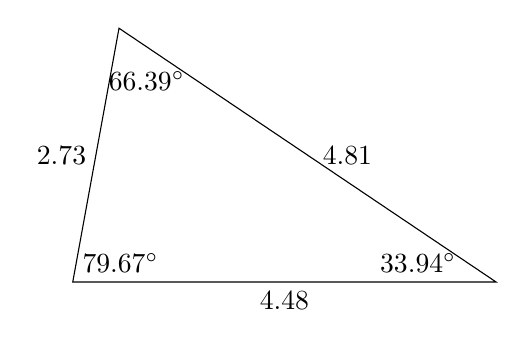
\begin{tikzpicture}[scale=1.2]
\coordinate (A1) at (0,0);
\coordinate (B1) at (4.48cm,0);
\coordinate (C1) at (79.67:2.73cm);
\node[above right] at (A1) {$79.67^\circ$};
\node[above left,xshift=-11pt] at (B1) {$33.94^\circ$};
\node[below,yshift=-12pt,xshift=10pt] at (C1) {$66.39^\circ$};
\draw (B1) -- node[below] {$4.48$} (A1) --
  node[left] {$2.73$} (C1) -- node[right,xshift=2pt] {$4.81$} cycle;
\end{tikzpicture}
\end{center}
\selectlanguage{hebrew}
\caption{משולש עם שטח והיקף שווה למשולש $(3,4,5)$}\label{f.not-a-right-triangle}
\end{figure}

\subsection*{מה ההפתעה?}

האם משלושים עם אותו שטח ואותו היקף חופפים? הרושם הראשון שלי היה "כן" כי לא קל למצוא דוגמאות נגדיות. מה שמפתיע הוא שנתון משולש שרירותי עם צלעות רציונליות, ניתן לבנות משולש לא-חופף עם אותו שטח והיקף למרות שהתוצאה יכולה להיות מוזרה כגון המשולשים
$(3,4,5)$
ו-%
$\left(\frac{156}{35}, \frac{101}{21}, \frac{41}{15}\right)$.


\subsection*{מקורות}

פרק זה מבוסס על 
\L{\cite{mccallum}}.
ברבש
\L{\cite{marita}}
מראה שאם נתון משולש שווה-צלעות, קיימים משולשים לא חופפים עם אותו היקף ואותו שטח, אולם ההוכחה שלה לא כוללת בנייה. 
